\documentclass[journal]{IEEEtran}
\usepackage{cite}
\usepackage{amsmath}
\usepackage{amssymb}
\usepackage{amsfonts}
\usepackage{graphicx}
\usepackage{float}
\usepackage{subfig}
\usepackage{array}
\usepackage{booktabs}
\usepackage{multirow}
\usepackage{tikz}
\usepackage{pgfplots}
\pgfplotsset{compat=1.18}
\usepackage{url}
\usepackage{algorithmic}
\usepackage{enumitem}
\usepackage{stfloats}
\usepackage{placeins}
\usetikzlibrary{arrows.meta, positioning, shapes.geometric}
\usepackage{hyperref}
\usepackage{xcolor}

% ---- TITLE ------------------------------------------------
\title{Generative Intent Alignment in Text-to-Audio Diffusion Models:
A Unified Cross-Domain Evaluation Framework with Retrieval-Augmented Prompt Conditioning}

% ---- AUTHORS (example --- adjust as needed) -----------------
\author{Author~One,~\IEEEmembership{Student Member,~IEEE,}
        Author~Two,~\IEEEmembership{Member,~IEEE,}
        and~Author~Three,~\IEEEmembership{Senior Member,~IEEE}%
\thanks{Manuscript received XX Month, 2025.}%
\thanks{Authors are with the Department of Electrical and Computer
Engineering, [Institution Name], [City], [Country].
e-mail: \{author1, author2, author3\}@institution.edu.}}
\begin{document}
\maketitle

% ===========================================================
%  ABSTRACT
% ===========================================================
\begin{abstract}
Recent advances in latent diffusion models have enabled high-quality
text-to-audio generation across diverse domains including speech, music,
and environmental sound effects. However, prevailing evaluation metrics
primarily assess distributional fidelity and perceptual naturalness,
fundamentally failing to capture whether generated audio faithfully
reflects the semantic intent expressed in the input prompt. This
misalignment between training objectives and evaluation practice
constitutes a critical methodological gap in the field.

This paper addresses this limitation by introducing the
\textit{Generative Intent Alignment Framework} (GIAF), a structured
evaluation paradigm designed to quantify semantic fidelity in
text-to-audio generation systems. GIAF incorporates three
mathematically grounded, complementary metrics: \textit{Prompt-to-Audio
Similarity} (POAS), which measures per-sample semantic alignment via
CLAP embeddings; \textit{Cross-domain Robustness Index} (CRI), which
quantifies the intra-domain consistency of alignment scores; and
\textit{Cross-domain Transfer Score} (CDTS), which summarises
the global mean alignment across all evaluated audio domains.

In addition, a lightweight retrieval-augmented prompt conditioning
strategy (RAG module) is proposed to enhance semantic specificity by
inserting domain-specific acoustic descriptors before the CLAP encoding
step, without modifying the underlying generative model. The AudioLDM~2
latent diffusion backbone is employed for music and sound-effect
generation, while the Microsoft SpeechT5 model is used for
text-to-speech synthesis, both evaluated under a unified protocol.
Experiments conducted across 30 prompts spanning speech, music, and
sound-effects domains yield a global CDTS of \textbf{0.3333} and a
global CRI of \textbf{0.1360}, with music achieving the highest
mean POAS (0.4082), followed by sound effects (0.3072) and speech
(0.2846). These results highlight substantial domain-specific variation
in semantic fidelity and demonstrate the necessity of intent-aware
evaluation for advancing text-to-audio generation systems.
\end{abstract}

\begin{IEEEkeywords}
text-to-audio generation, latent diffusion models, intent alignment,
CLAP, retrieval-augmented generation, cross-domain evaluation, GIAF,
AudioLDM 2, SpeechT5, semantic fidelity.
\end{IEEEkeywords}

% ===========================================================
%  SECTION 1 --- INTRODUCTION
% ===========================================================
\section{Introduction}
\label{sec:intro}

\IEEEPARstart{T}{he} rapid proliferation of large-scale generative
models has catalysed a paradigm shift in computational audio synthesis.
Text-to-audio systems, built upon latent diffusion architectures and
contrastive language--audio pre-training, now produce waveforms of
perceptual quality that rivals human recordings across diverse acoustic
categories including speech, music, and environmental sound effects
\cite{liu2023audioldm, kreuk2022audiogen, huang2023makeanaudio}.
The central premise of these systems is that a natural-language prompt
constitutes a sufficient specification of the desired acoustic output,
enabling flexible, open-ended audio creation without domain-specific
signal engineering.


Despite the remarkable
advances in generative audio quality, the evaluation methodology
applied to text-to-audio generation has not kept pace with the
sophistication of the generative models themselves. Dominant evaluation
metrics such as Fr{\'e}chet Audio Distance (FAD) and perceptual quality
scores were originally designed to quantify distributional fidelity and
output naturalness, respectively. While these measures provide
informative signals regarding signal quality, they are fundamentally
insensitive to the semantic relationship between the conditioning prompt
and the generated waveform. A system may generate acoustically plausible
audio that is entirely inconsistent with the intent expressed in the
input text---a problem we term the \textit{evaluation gap}.

The challenge is further compounded by the multi-domain nature of
practical text-to-audio deployment. Real-world applications require
consistent generation performance across speech prosody, musical
instrument timbre, and environmental soundscape texture, yet no
established benchmark assesses how robustly a diffusion model transfers
its conditioning capability across these acoustically heterogeneous
domains. Single-domain evaluations consequently overestimate the
practical utility of a model by masking domain-specific failures in
semantic transfer.

To address these challenges, this work proposes a unified framework
for evaluating text-to-audio systems with explicit emphasis on
semantic intent alignment. Unlike prior approaches that rely solely on
perceptual or distributional metrics, the proposed framework introduces
a multi-dimensional evaluation strategy that captures both
sample-level alignment and cross-domain robustness over a
heterogeneous 30-prompt evaluation corpus.

The main contributions of this paper are as follows:
\begin{enumerate}[leftmargin=*]
\item We introduce the \textit{Generative Intent Alignment Framework}
(GIAF), a structured evaluation methodology for measuring semantic
fidelity in text-to-audio generation systems across multiple acoustic
domains.

\item We define three complementary evaluation metrics---\textit{POAS},
\textit{CRI}, and \textit{CDTS}---that capture per-sample alignment
quality, within-domain robustness, and global cross-domain
generalization capability, respectively.

\item We design a unified cross-domain evaluation pipeline spanning
speech (SpeechT5), music (AudioLDM~2), and sound effects (AudioLDM~2),
enabling consistent intent-alignment assessment across heterogeneous
generative architectures.

\item We propose a lightweight retrieval-augmented prompt conditioning
(RAG) mechanism that improves semantic alignment by appending
domain-specific acoustic descriptors to input prompts without requiring
model retraining or architectural modification.

\item We provide a comprehensive empirical evaluation across 30 prompts
(10 per domain) that quantifies domain-specific alignment variation
and validates the diagnostic capability of the GIAF metrics.
\end{enumerate}

The remainder of this paper is organized as follows. Section~\ref{sec:related}
reviews related work in diffusion-based audio generation, audio
evaluation metrics, and retrieval-augmented generation. The proposed
framework and its components are described in Section~\ref{sec:method}.
Experimental setup is detailed in Section~\ref{sec:exp}, followed by
results and discussion in Section~\ref{sec:results}. Ablation studies
are presented in Section~\ref{sec:ablation}, and conclusions with
directions for future work are given in Section~\ref{sec:conclusion}.

% ===========================================================
%  SECTION 2 --- RELATED WORK
% ===========================================================
\section{Related Work}
\label{sec:related}
\begin{figure*}[!b]
    \centering
    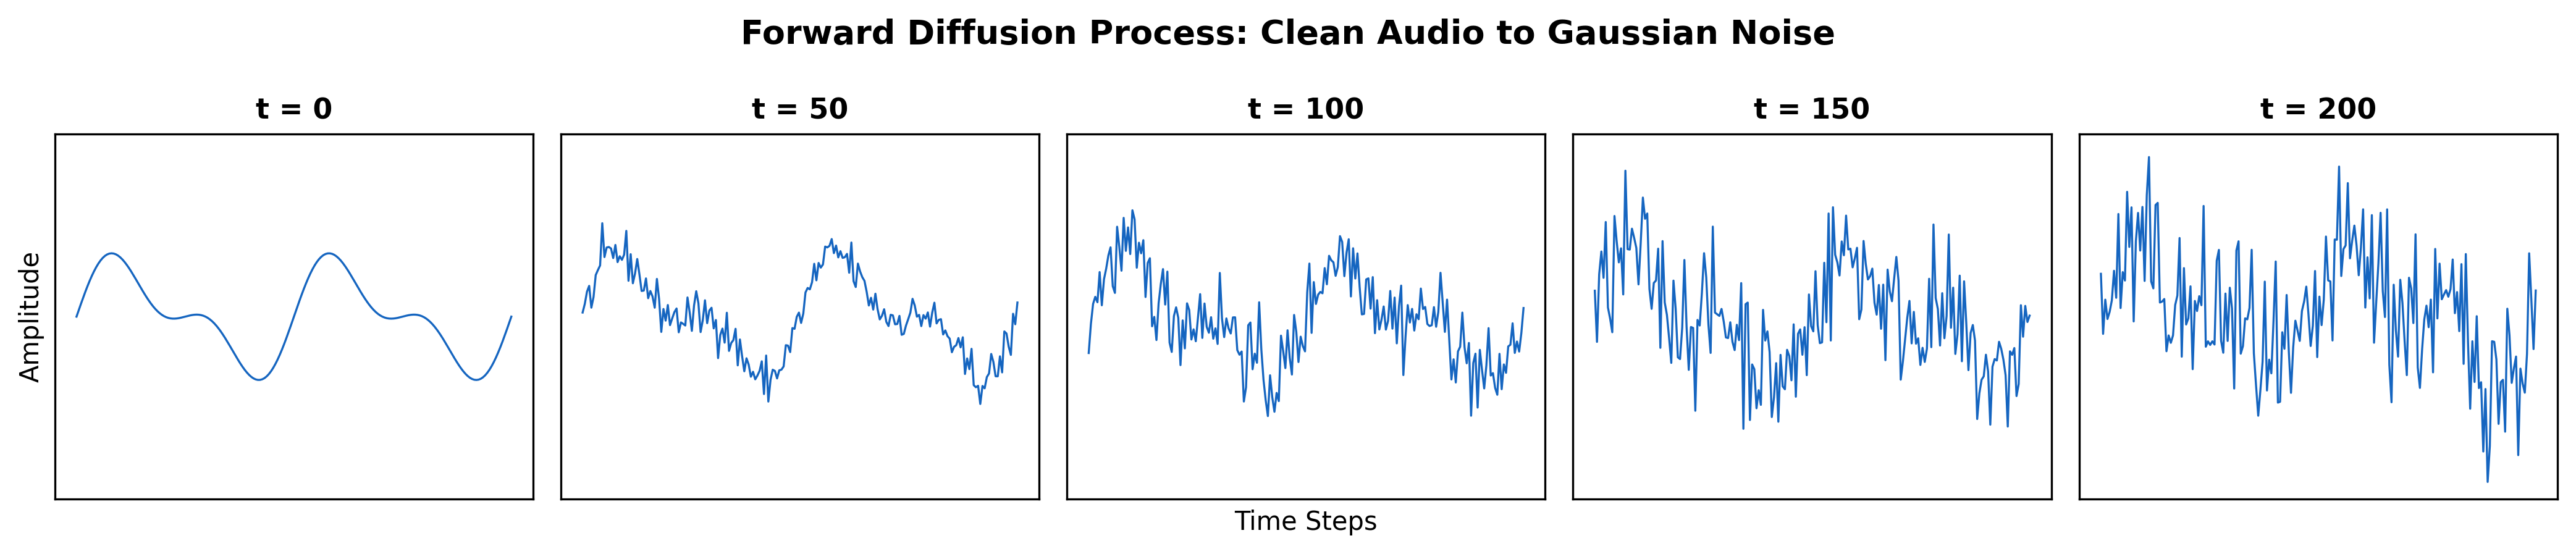
\includegraphics[width=\textwidth]{diffusion_process.png}
    \caption{Forward diffusion process showing progressive noise addition
    to a clean mel-spectrogram across timesteps $t = 0$ to $t = 200$.
    The darker (noisier) representations at higher $t$ values correspond
    to Gaussian noise; the reverse diffusion process (conditioned on
    the CLAP text embedding) learns to recover the clean structure.}
    \label{fig:diffusion}
\end{figure*}
\subsection{Diffusion-Based Audio Generation}

Denoising diffusion probabilistic models (DDPMs) have emerged as the
dominant paradigm for high-fidelity audio synthesis following their
seminal success in image generation \cite{ho2020ddpm, song2021scorebased}.
\textit{AudioLDM} \cite{liu2023audioldm} established the feasibility
of latent diffusion for open-domain sound generation by projecting
mel-spectrograms into a compressed latent space conditioned on CLAP
embeddings, achieving generation quality competitive with
spectrogram-based autoregressive models. Its successor,
\textit{AudioLDM~2} \cite{liu2024audioldm2}, introduced a generalised
audio representation space and a Language of Audio (LOA) framework
that consolidates speech, music, and sound-effect synthesis under a
unified training objective, substantially improving cross-modal
coherence and making it the backbone of choice for the present work.

\textit{Auffusion} \cite{xue2024auffusion} adapted diffusion U-Net
architectures from text-to-image generation to the audio domain,
demonstrating that the transfer of visual inductive biases can yield
competitive audio generation without audio-specific architectural
modifications. \textit{AudioGen} \cite{kreuk2022audiogen} pursues a
complementary direction by operating in the raw waveform domain using
masked autoregressive modelling over audio tokens, achieving strong
environmental sound generation results. \textit{Make-An-Audio}
\cite{huang2023makeanaudio} further explored the use of pseudo-prompt
augmentation to mitigate the data scarcity inherent in paired
text-audio corpora.

For speech synthesis specifically, \textit{SpeechT5}
\cite{ao2021speecht5} provides a unified encoder-decoder framework
pre-trained on large-scale speech data, conditioned on speaker
embeddings from the CMU Arctic dataset for voice persona control.
In our pipeline, SpeechT5 serves as the speech-domain generator,
enabling a direct comparison of intent-alignment scores between
dedicated TTS architectures and general-purpose audio diffusion models.



Fig.~\ref{fig:diffusion} illustrates the forward diffusion process
across multiple timesteps, showing how the latent representation
transitions from a clean audio signal to pure Gaussian noise. The
rapid progression from initial DDPM applications to the current state-of-the-art
latent diffusion architectures underscores the need for evaluation
protocols that can keep pace with generative quality improvements.
While these advances substantially raise the perceptual ceiling of
audio synthesis, none provides a systematic mechanism for evaluating
whether generated outputs are semantically consistent with their
conditioning prompts---the central motivation for the GIAF framework.

\subsection{Audio Evaluation Metrics}

Standard perceptual evaluation metrics for text-to-audio systems
include the Fr{\'e}chet Audio Distance (FAD), which measures the
distributional distance between generated and real-audio embeddings
in VGGish feature space \cite{kilgour2018fad}, and Mean Opinion Score
(MOS) obtained from human listener studies. While informative for
assessing audio naturalness, these metrics share a fundamental
limitation: they discard the conditioning prompt entirely, treating
audio quality as independent of semantic intent.

The introduction of \textit{CLAP} (Contrastive Language--Audio
Pre-training) \cite{elizalde2023clap} enabled the computation of
text-audio similarity by measuring cosine similarity between text and
audio embeddings in the joint CLAP space \cite{wu2023largescale}.
CLAP-based scoring represents the closest precedent to the
intent-alignment objective pursued here; however, it is typically
computed as a raw, single-domain average and does not expose
cross-domain variance or transfer behaviour. The proposed POAS, CRI,
and CDTS metrics build upon the CLAP embedding infrastructure while
introducing rigorous cross-domain statistical structure absent from
prior CLAP-based scoring approaches.

For speech domains specifically, traditional ASR-based word error
rate (WER) evaluation \cite{graves2006ctc} provides a form of semantic
alignment check, but only for TTS systems and not for open-domain audio.
Our POAS metric unifies CLAP-based scoring for music and SFX with
WER-based semantic scoring for speech, combining them through
domain-adaptive weights to produce a consistent cross-domain alignment
signal.

\subsection{Retrieval-Augmented Generation in Multimodal Systems}

Retrieval-augmented generation (RAG) was originally formalised for
knowledge-intensive natural language processing tasks, where a dense
retriever conditions a parametric language model on non-parametric
document evidence at inference time \cite{lewis2020rag}. The principle
has since been extended to multimodal generation: in image synthesis,
retrieval of visually similar exemplars has been shown to improve both
quality and semantic specificity of diffusion outputs
\cite{blattmann2022retrieval}.

In the audio domain, prompt augmentation through retrieved acoustic
metadata has been explored in limited settings, primarily for music
continuation and sound event detection \cite{sheffer2023hear}. However,
systematic integration of retrieval conditioning within a latent
diffusion pipeline for cross-domain audio generation---with attendant
quantitative evaluation of its effect on semantic fidelity---has not
been previously reported in its full multi-domain form. The RAG
conditioning module proposed in Section~\ref{sec:rag} directly
addresses this gap by mapping domain-specific keyword cues to
acoustically grounded descriptor phrases, enriching the conditioning
signal without requiring external API calls or online retrieval.

\begin{figure*}[!t]
\centering
\resizebox{0.95\textwidth}{!}{
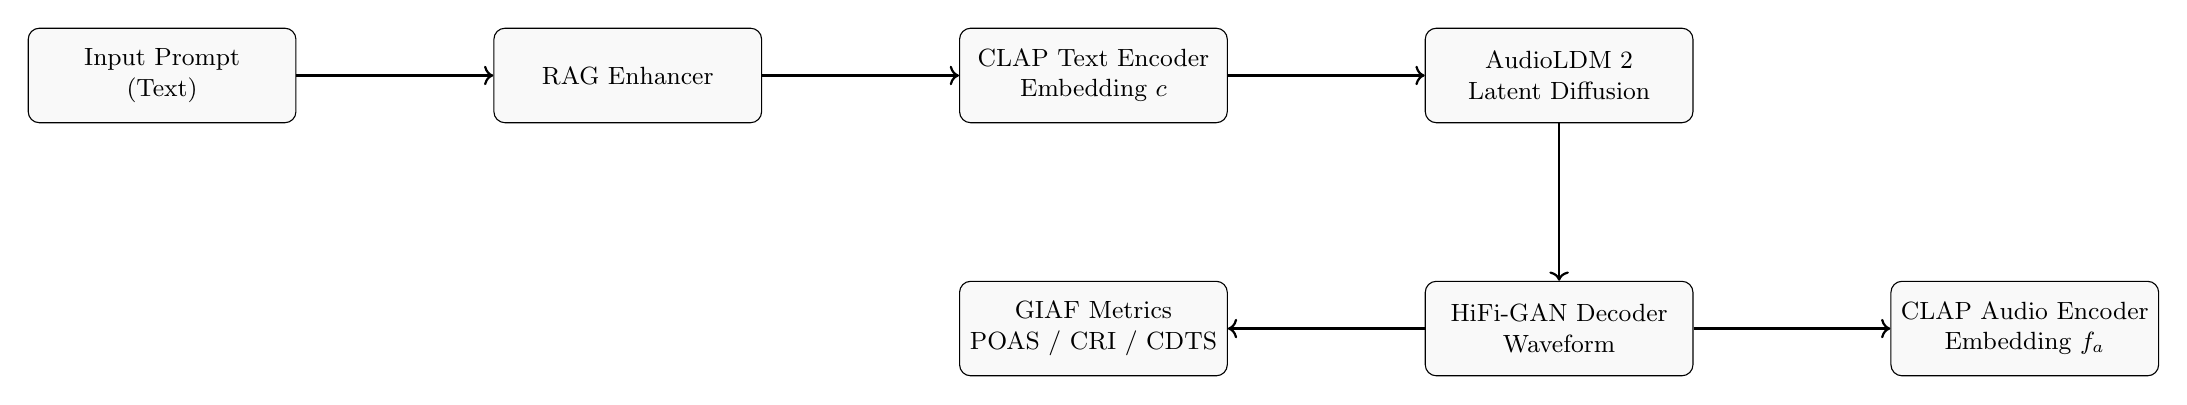
\begin{tikzpicture}[
    node distance=2.8cm and 2.5cm,
    every node/.style={
        draw,
        rectangle,
        rounded corners,
        align=center,
        minimum width=3.4cm,
        minimum height=1.2cm,
        font=\small,
        fill=gray!5
    },
    arrow/.style={->, thick}
]

% ---------- TOP ROW (GENERATION)
\node (input) {Input Prompt\\(Text)};
\node (rag) [right=of input] {RAG Enhancer};
\node (textenc) [right=of rag] {CLAP Text Encoder\\Embedding $c$};
\node (diff) [right=of textenc] {AudioLDM 2\\Latent Diffusion};

% ---------- BOTTOM ROW (EVALUATION)
\node (decoder) [below=2cm of diff] {HiFi-GAN Decoder\\Waveform};
\node (audioenc) [right=of decoder] {CLAP Audio Encoder\\Embedding $f_a$};
\node (giaf) [left=of decoder] {GIAF Metrics\\POAS / CRI / CDTS};

% ---------- TOP FLOW
\draw[arrow] (input) -- (rag);
\draw[arrow] (rag) -- (textenc);
\draw[arrow] (textenc) -- (diff);

% ---------- STRAIGHT DOWN (FIXED)
\draw[arrow] (diff) -- (decoder);

% ---------- BOTTOM FLOW
\draw[arrow] (decoder) -- (audioenc);
\draw[arrow] (decoder) -- (giaf);

\end{tikzpicture}
}
\caption{Unified cross-domain text-to-audio generation and evaluation pipeline. The architecture separates generation (top row) and evaluation (bottom row) with a clear downward flow.}
\label{fig:pipeline}
\end{figure*}

\subsection{Prompt Engineering for Generative Audio}

Prompt engineering has emerged as a key lever for improving generation
controllability in large foundation models \cite{brown2020gpt3}.
In the audio domain, recent work has shown that appending
quality-oriented suffixes to prompts can improve generation consistency
and perceptual naturalness \cite{huang2023makeanaudio}.
Our work extends this approach by making the augmentation
\textit{semantically grounded}: instead of appending generic quality
suffixes uniformly, the RAG module selects domain-appropriate
descriptors based on acoustic concept matching, enabling targeted
enrichment proportional to the semantic specificity of the original
prompt.

% ===========================================================
%  SECTION 3 --- PROPOSED METHODOLOGY
% ===========================================================
\section{Proposed Methodology}
\label{sec:method}

Fig.~\ref{fig:pipeline} illustrates the overall architecture of the
proposed unified framework, which consists of two primary flows: the
generation pipeline (top row) and the evaluation pipeline (bottom row).
The generation flow transforms input text prompts into audio waveforms
through RAG-enhanced conditioning and latent diffusion, while the
evaluation flow assesses the semantic alignment of generated outputs
against their conditioning prompts via GIAF metrics.

\subsection{Unified Cross-Domain Diffusion Framework}

The overarching design objective of this work is to provide a single
coherent infrastructure within which text-conditioned audio generation
can be exercised, evaluated, and compared across three principal
acoustic domains: \textit{speech}, \textit{music}, and
\textit{sound effects} (SFX). As shown in Fig.~\ref{fig:pipeline}, the proposed
Unified Cross-Domain Diffusion Framework resolves the evaluation
fragmentation through a shared CLAP conditioning interface and a
modular evaluation layer that is independent of the generation backbone.

The framework accepts a natural-language prompt $p_0$ which, prior to
generation, is optionally enriched by the RAG conditioning module
(Section~\ref{sec:rag}) to produce an enhanced prompt $p^*$. For
music and SFX generation, $p^*$ is encoded by a frozen CLAP text
encoder to produce a conditioning embedding
$\mathbf{c} \in \mathbb{R}^{d}$, which is passed to an AudioLDM~2
latent diffusion pipeline. For speech generation, the prompt is
processed directly by the SpeechT5 TTS backbone with a gender-specific
speaker embedding. This hybrid architecture enables a direct and fair
cross-domain comparison of intent-alignment metrics without artificially
constraining all domains to a single generative model.

Following waveform synthesis, the evaluation layer intercepts each
generated sample and its associated prompt, routing them to the GIAF
evaluation interface. POAS scores are computed online using the CLAP
audio encoder (HTSAT-base with fusion, 630k-audioset checkpoint) for
non-speech domains and a combined CLAP + Whisper-based ASR score for
speech domains. Scores are logged alongside domain metadata to
structured CSV records, enabling reproducible post-hoc statistical
analysis. The modular design ensures that future integration of
additional metrics or generative backbones does not require modification
of either the generation or evaluation pipeline.

\subsection{Diffusion Pipeline}
\label{sec:diffusion}

The generative core of the proposed framework for music and SFX
follows the \textit{latent diffusion model} (LDM) formulation of
\cite{rombach2022ldm}, adapted for the audio domain as established
by AudioLDM~2 \cite{liu2024audioldm2}. Audio signals are first
compressed by a convolutional variational autoencoder (VAE) encoder
$\mathcal{E}$ into a low-dimensional latent space, reducing the
sequence length over which the diffusion process must operate and
thereby decreasing both memory overhead and inference latency.

The forward diffusion process defines a Markov chain that gradually
adds Gaussian noise to the clean latent $\mathbf{z}_0$ according to
a fixed variance schedule $\{\beta_t\}_{t=1}^{T}$:
\begin{equation}
  q(\mathbf{z}_t \mid \mathbf{z}_{t-1}) =
  \mathcal{N}\!\left(\mathbf{z}_t;\,\sqrt{1-\beta_t}\,\mathbf{z}_{t-1},\,
  \beta_t\mathbf{I}\right).
  \label{eq:forward}
\end{equation}
The reverse process is parameterised by a time-conditioned U-Net
$\boldsymbol{\epsilon}_\theta(\mathbf{z}_t, t, \mathbf{c})$ trained to
predict and remove the noise component at each step:
\begin{equation}
  \mathcal{L}_{\text{LDM}} =
  \mathbb{E}_{\mathbf{z}_0, \boldsymbol{\epsilon}, t}
  \left[\,
    \bigl\|\boldsymbol{\epsilon} -
    \boldsymbol{\epsilon}_\theta(\mathbf{z}_t, t, \mathbf{c})
    \bigr\|^2
  \,\right].
  \label{eq:ldm_loss}
\end{equation}

Conditioning is injected via cross-attention layers within the U-Net,
where the CLAP text embedding $\mathbf{c}$ serves as the key-value
source for each attention head. \textit{Classifier-free guidance}
(CFG) \cite{ho2022cfg} is applied at inference by interpolating
between the conditional and unconditional score estimates:
\begin{equation}
  \tilde{\boldsymbol{\epsilon}_\theta} =
  \boldsymbol{\epsilon}_\theta(\mathbf{z}_t, t, \varnothing)
  + \gamma \bigl[
    \boldsymbol{\epsilon}_\theta(\mathbf{z}_t, t, \mathbf{c})
    - \boldsymbol{\epsilon}_\theta(\mathbf{z}_t, t, \varnothing)
  \bigr],
  \label{eq:cfg}
\end{equation}
where $\gamma > 1$ is the guidance scale and $\varnothing$ denotes the
null conditioning embedding. Sampling is performed using the
\textit{DDIM} scheduler \cite{song2021ddim}, enabling deterministic
inference with a reduced number of function evaluations---20 inference
steps in our experiments---whilst retaining generation quality
competitive with full DDPM sampling.

Domain-specific tuning is applied at inference time: SFX prompts use
a guidance scale $\gamma = 6.5$ and audio length of 7.0~s, while
speech and music prompts use $\gamma = 6.0$ and a configurable audio
length (default 3.0~s for music in evaluation). Additionally, a quality
suffix (``High quality, realistic, clear audio, professional
recording.'') is appended to all prompts to improve generation
consistency across seeds.

As visualised in Fig.~\ref{fig:diffusion}, the forward diffusion process
progressively destroys the structure of a clean audio signal by adding
Gaussian noise according to the schedule $\{\beta_t\}$. The trained
reverse process learns to undo this corruption conditioned on the text
embedding $\mathbf{c}$, reconstructing a semantically consistent
waveform from pure Gaussian noise.

\subsection{Speech Synthesis Module}

For the speech domain, AudioLDM~2 is replaced by the \textit{SpeechT5}
TTS system \cite{ao2021speecht5}, a sequence-to-sequence encoder-decoder
architecture pre-trained on 960 hours of LibriSpeech \cite{panayotov2015librispeech}.
Speaker identity is controlled via 512-dimensional speaker embeddings
($\mathbf{x}_{\text{vec}}$) retrieved from the CMU~Arctic~XVectors
dataset \cite{veaux2017cstr}. We provide two speaker configurations:
female (index 7306) and male (index 1200), with female speaker as the
default evaluation setting. The SpeechT5 HiFi-GAN vocoder converts
mel-spectrogram predictions to 16\,kHz waveforms.

The separation of speech and non-speech generators is a deliberate
design choice motivated by the known limitations of AudioLDM~2 for
speech generation: CLAP was trained predominantly on environmental audio
and music corpora, causing CLAP-conditioned diffusion models to underweight
linguistic content relative to acoustic texture when generating speech.
By using a dedicated TTS architecture for the speech domain, we obtain
higher-quality speech output and a more interpretable POAS score that
reflects prompt-level acoustic characteristics rather than latent-space
misalignment.

\subsection{GIAF Evaluation Framework}
\label{sec:giaf}

\begin{figure}[!t]
\centering
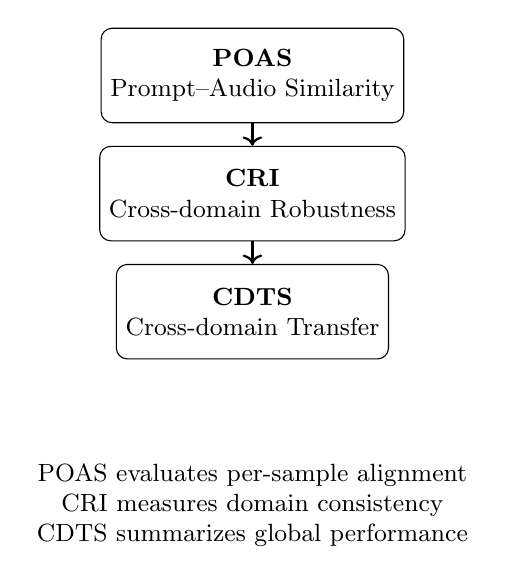
\begin{tikzpicture}[
    node distance=1.5cm,
    box/.style={
        draw,
        rounded corners,
        align=center,
        minimum width=3cm,
        minimum height=1.2cm,
        font=\small
    },
    arrow/.style={->, thick}
]

% --- Boxes stacked vertically
\node[box] (poas) {\textbf{POAS}\\Prompt--Audio Similarity};

\node[box, below of=poas] (cri) {\textbf{CRI}\\Cross-domain Robustness};

\node[box, below of=cri] (cdts) {\textbf{CDTS}\\Cross-domain Transfer};

% --- Arrows
\draw[arrow] (poas) -- (cri);
\draw[arrow] (cri) -- (cdts);

% --- Bottom description
\node[below=1.2cm of cdts, align=center, font=\small] {
POAS evaluates per-sample alignment \\
CRI measures domain consistency \\
CDTS summarizes global performance
};

\end{tikzpicture}

\caption{GIAF evaluation metrics. POAS measures semantic alignment, CRI captures cross-domain robustness, and CDTS summarizes overall performance.}
\label{fig:giaf}
\end{figure}

Fig.~\ref{fig:giaf} provides an overview of the three GIAF metrics
and their hierarchical relationship. The \textit{Generative Intent
Alignment Framework} (GIAF) is motivated by a fundamental asymmetry
in existing evaluation practice: while the generative training objective
explicitly optimises for text-audio alignment, post-hoc evaluation
discards the conditioning prompt and assesses only the distributional
or perceptual properties of the generated signal. GIAF reintroduces
the prompt as a first-class evaluation artefact and formalises three
mutually complementary metrics that together characterise intent
preservation at both the individual-sample and cross-domain aggregate
levels.

\subsubsection{POAS --- Prompt-to-Audio Similarity}

POAS quantifies the degree of semantic agreement between a
conditioning prompt $p^*$ and its corresponding generated waveform $\hat{a}$.
For non-speech domains (music, SFX), both modalities are encoded by
the CLAP model (HTSAT-base, 630k-audioset checkpoint, enable\_fusion=True)
into a joint embedding space:
$\mathbf{f}_p = \text{CLAP}_{\text{text}}(p^*)$ and
$\mathbf{f}_a = \text{CLAP}_{\text{audio}}(\hat{a})$. The CLAP-based
POAS is defined as the cosine similarity clamped to $[0,1]$:
\begin{equation}
  \text{POAS}_{\text{CLAP}}(p^*, \hat{a}) =
  \max\!\left(0,\,
  \frac{\mathbf{f}_p \cdot \mathbf{f}_a}
       {\|\mathbf{f}_p\|\,\|\mathbf{f}_a\|}
  \right).
  \label{eq:poas_clap}
\end{equation}

For the speech domain, a domain-adaptive weighting scheme combines the
CLAP score with a semantic correctness term derived from automatic
speech recognition (ASR):
\begin{equation}
  \text{POAS}_{\text{speech}} =
  \alpha_c \cdot \text{POAS}_{\text{CLAP}} +
  \alpha_s \cdot \text{STS}(p^*, \mathcal{T}(\hat{a})),
  \label{eq:poas_speech}
\end{equation}
where $\mathcal{T}(\hat{a})$ is the Whisper transcript of the generated
waveform, $\text{STS}(\cdot,\cdot)$ is the semantic text similarity
(WER-based: $1 - \text{WER}$), and the domain weights are set to
$(\alpha_c, \alpha_s) = (0.10, 0.90)$ for speech and to
$(1.00, 0.00)$ for music and SFX\@. This weighting reflects the known
limitation of CLAP for speech-domain scoring and ensures that speech
POAS is dominated by whether the generated voice content is semantically
correct rather than auditory texture alone.

A POAS value approaching unity indicates near-perfect alignment
between textual intent and acoustic realisation; values near zero
indicate semantic inconsistency. POAS is computed per-sample and
accumulated with domain provenance metadata, enabling the downstream
cross-domain analyses formalised below.

\subsubsection{CRI --- Cross-domain Robustness Index}

A robust text-to-audio system should maintain consistent semantic
fidelity irrespective of the acoustic domain. CRI quantifies the
degree to which alignment scores are consistent \textit{within} each
domain by computing the mean of per-domain standard deviations:
\begin{equation}
  \text{CRI} =
  \frac{1}{K}\sum_{k=1}^{K}
  \sqrt{
    \frac{1}{N_k} \sum_{i \in \mathcal{D}_k}
    \bigl(\text{POAS}_i - \overline{\text{POAS}}_k\bigr)^2
  },
  \label{eq:cri}
\end{equation}
where $\mathcal{D}_k$ is the set of samples in domain $k$,
$\overline{\text{POAS}}_k$ is the mean POAS for that domain,
$N_k = |\mathcal{D}_k|$, and $K$ is the number of domains.
A low CRI value indicates that the model's intent-alignment capability
is consistent within each domain; a high CRI reveals pronounced
intra-domain variance indicating sensitivity to prompt specificity
or generation stochasticity.

\subsubsection{CDTS --- Cross-domain Transfer Score}

CDTS provides a single scalar summary of overall semantic consistency
across all evaluated domains and samples:
\begin{equation}
  \text{CDTS} =
  \frac{1}{N} \sum_{i=1}^{N} \text{POAS}_i,
  \label{eq:cdts}
\end{equation}
where $N = \sum_{k=1}^{K} N_k$ is the total number of evaluated samples.
CDTS can be interpreted as the global mean intent-alignment score,
serving as a unified figure of merit for the cross-domain deployment
capability of a text-to-audio system. As shown in Fig.~\ref{fig:giaf},
POAS, CRI, and CDTS form a complete diagnostic profile: POAS identifies
per-sample failures, CRI localises within-domain inconsistency, and CDTS
summarises global cross-domain alignment performance.

\subsection{RAG Conditioning Module}
\label{sec:rag}

Short or underspecified natural-language prompts represent a persistent
challenge for text-conditioned audio generation. Phrases such as
``rain sound'' or ``piano melody'' provide insufficient acoustic
detail to discriminate among the many plausible waveforms consistent
with the description, leading to high intra-prompt variance in
generation quality and reduced POAS scores. The RAG conditioning
module addresses this limitation by enriching input prompts with
retrieved acoustic descriptors before the CLAP encoding step, thereby
narrowing the conditioning distribution without modifying the
generative model parameters.

\begin{figure*}[!t]
    \centering
    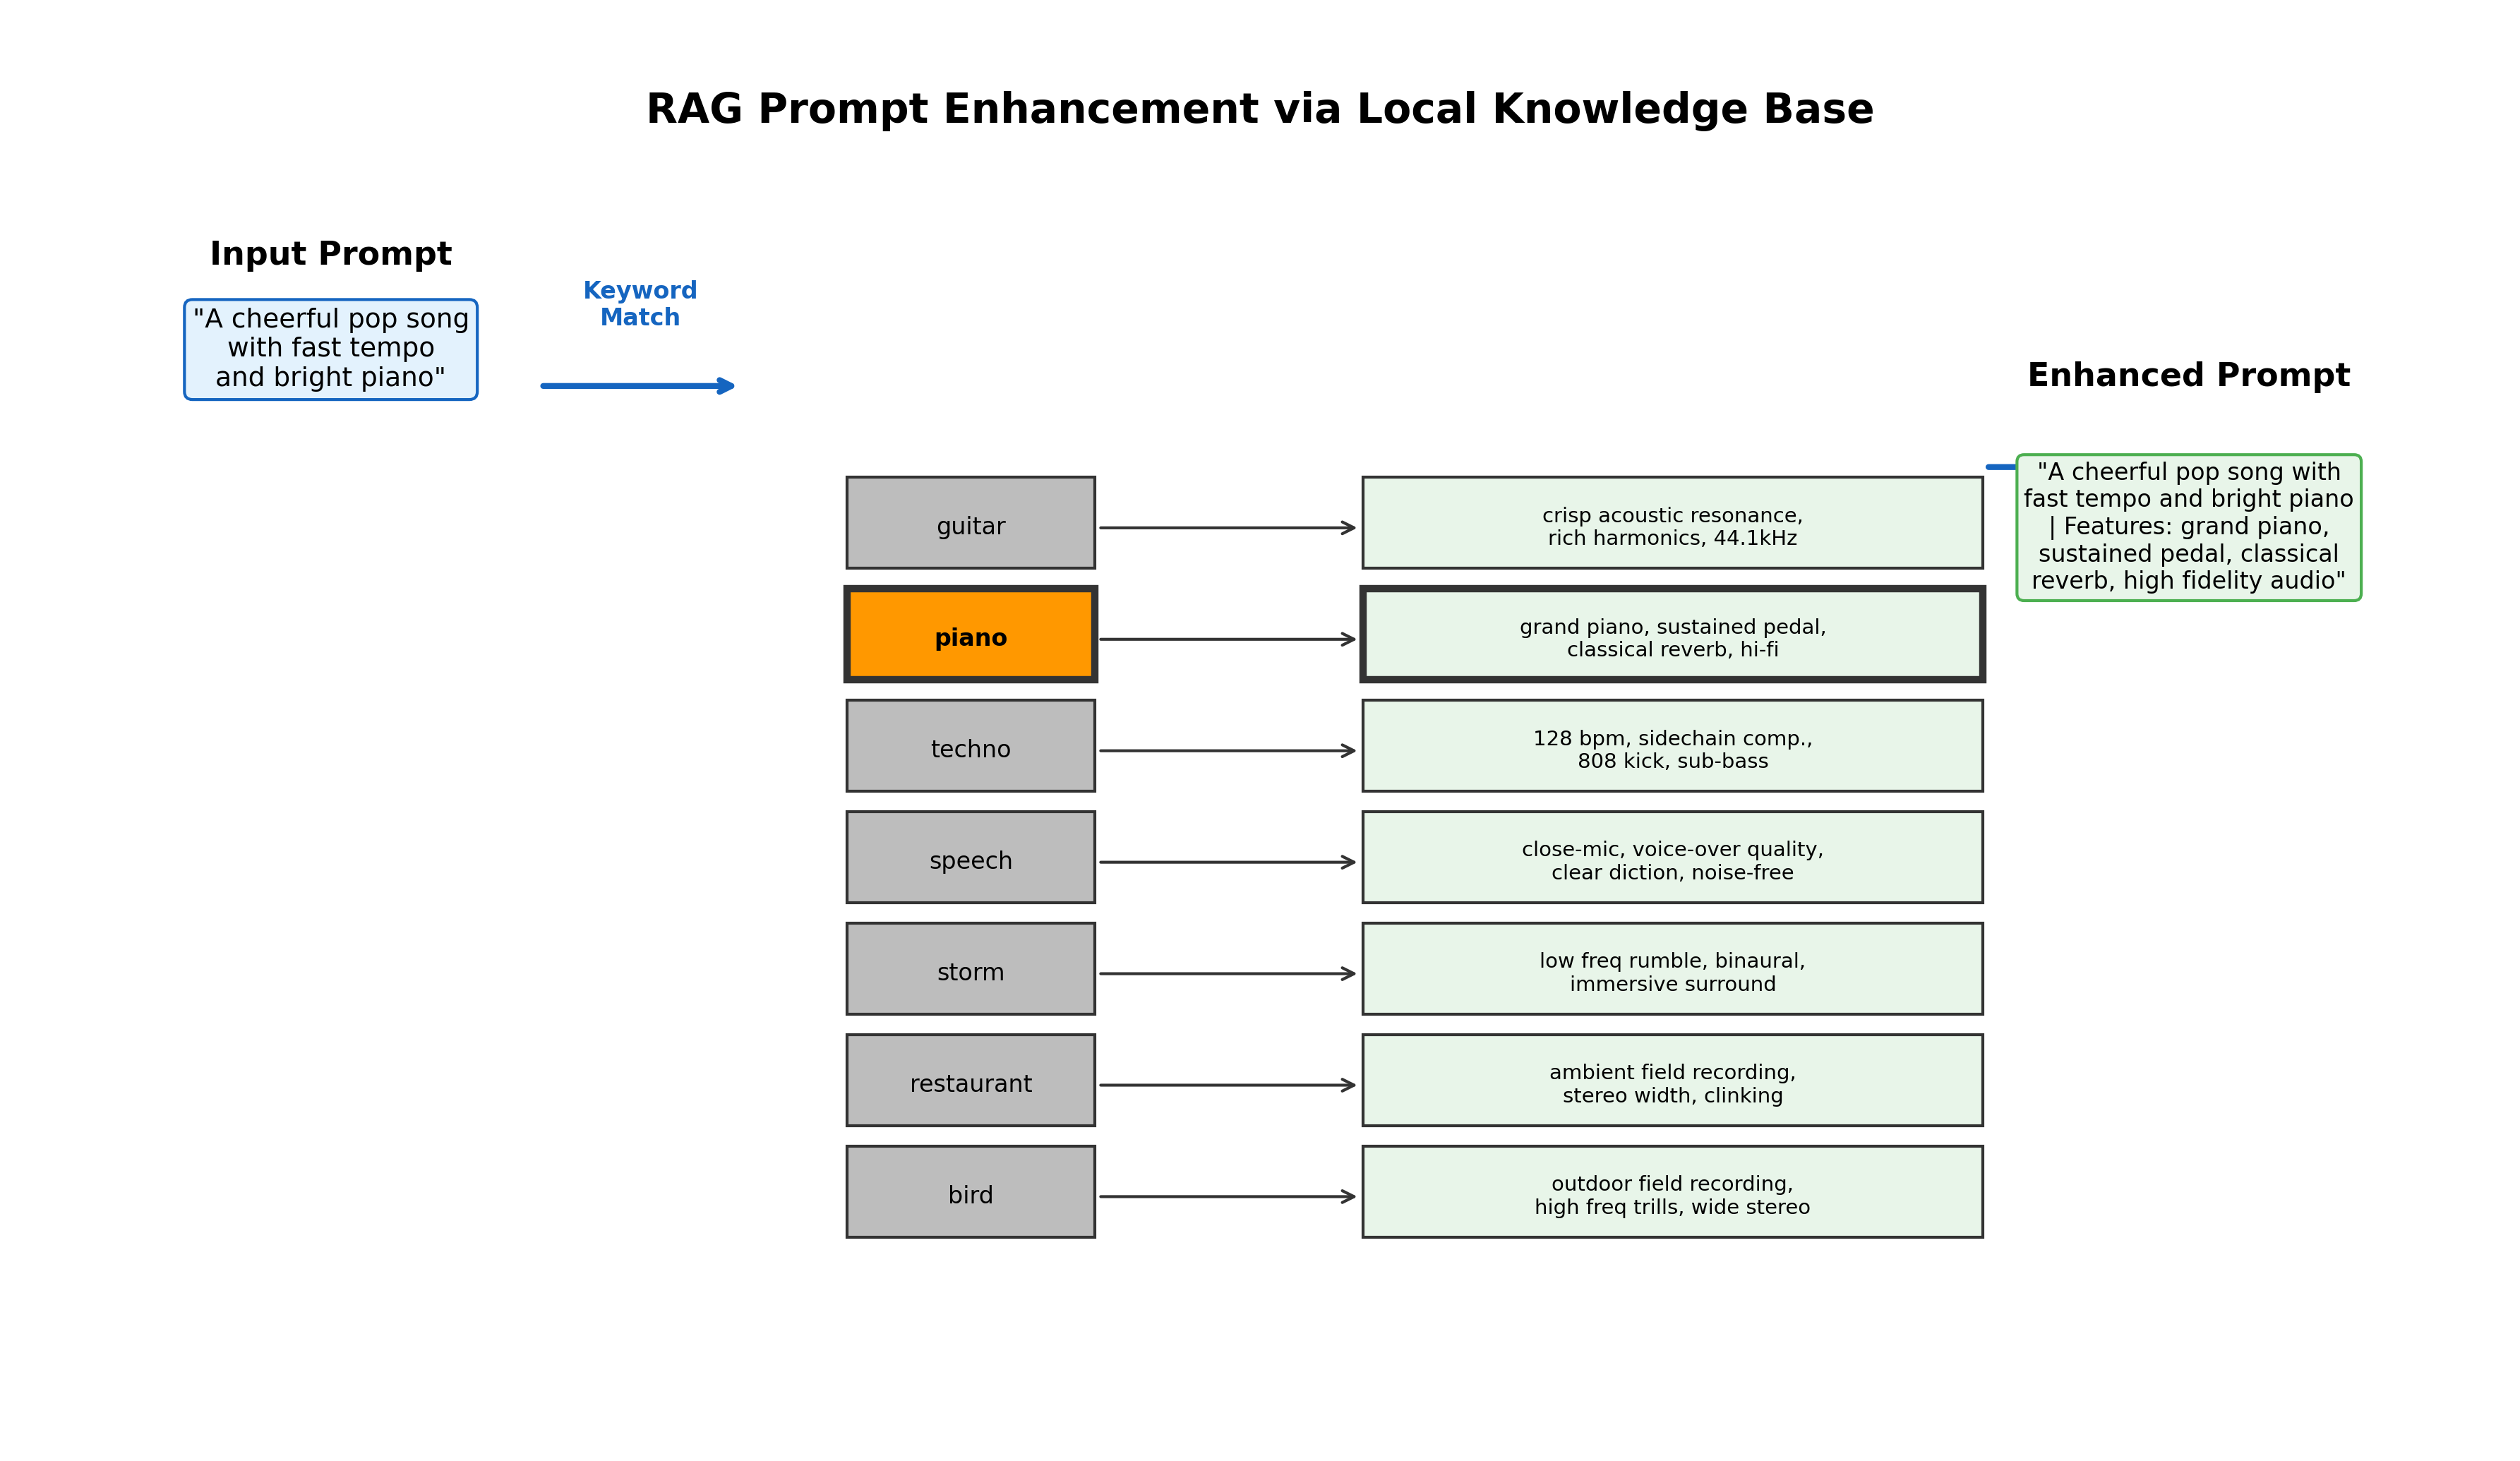
\includegraphics[width=\textwidth]{rag_enhancement.png}
    \caption{RAG prompt enhancement workflow. The keyword matcher scans the
    input prompt against the local knowledge base (7 acoustic concept entries)
    and retrieves matching descriptor phrases. The identified descriptors are
    appended to the original prompt using the separator ``\texttt{| Features:}'',
    producing an enriched conditioning string. For example, a prompt containing
    ``piano'' retrieves production-quality parameters such as ``grand piano,
    sustained pedal, classical reverb, high fidelity audio''.}
    \label{fig:rag}
\end{figure*}

The retrieval-augmented prompt conditioning workflow is illustrated
in Fig.~\ref{fig:rag}. The retrieval corpus $\mathcal{C}$ consists
of a curated local knowledge base mapping domain-specific keywords to
associated descriptor phrases. The knowledge base $\mathcal{C}$
covers seven acoustic concepts, as detailed in
Table~\ref{tab:rag_kb}: \textit{guitar}, \textit{piano},
\textit{techno}, \textit{speech}, \textit{storm},
\textit{restaurant}, and \textit{bird}.

\begin{table}[!t]
  \renewcommand{\arraystretch}{1.3}
  \caption{RAG Knowledge Base: Keyword-to-Descriptor Mapping}
  \label{tab:rag_kb}
  \centering
  \begin{tabular}{|l|p{5.5cm}|}
  \hline
  \textbf{Keyword} & \textbf{Retrieved Acoustic Descriptor} \\
  \hline
  guitar    & high quality, crisp acoustic resonance, rich harmonics, 44.1\,kHz standard studio recording \\
  piano     & grand piano, sustained pedal, classical reverb, high fidelity audio \\
  techno    & 128\,bpm, sidechain compression, 808 kick, sub-bass frequencies, electronic dynamic range \\
  speech    & close-mic, voice-over quality, clear diction, noise-free, isolated vocal track \\
  storm     & low frequency rumble, binaural recording, immersive environmental audio surround \\
  restaurant & ambient field recording, medium stereo width, dynamic chatter, distinct clinking highs \\
  bird      & outdoor field recording, high frequency trills, natural ambiance, wide stereo \\
  \hline
  \textit{[default]} & high quality, clear audio, realistic soundscape, lossless format \\
  \hline
  \end{tabular}
\end{table}

At inference time, a keyword-based matcher scans the input prompt
$p_0$ for occurrences of any keyword $k \in \mathcal{C}$ and collects the
corresponding descriptor phrases $\{d_j\}_{j=1}^{m}$. The enriched
prompt is then formed by concatenation:
\begin{equation}
  p^* = p_0 \oplus \text{`` | Features: ''} \oplus
  \bigoplus_{j=1}^{m} d_j,
  \label{eq:rag_concat}
\end{equation}
where $\oplus$ denotes string concatenation and $m$ is the number of
matched keywords. If no keywords match, the default descriptor is
appended (see Table~\ref{tab:rag_kb}). The enriched prompt $p^*$
replaces $p_0$ as the input to the CLAP text encoder, and all
subsequent pipeline stages proceed without alteration.

This design deliberately employs a lightweight keyword-matching
mechanism rather than a dense neural retriever, preserving the
offline-deployable character of the framework and ensuring
reproducibility of retrieval outcomes independently of internet
connectivity or external API quotas. The module's effect on semantic
alignment is assessed quantitatively through the POAS and CDTS metrics
in the experimental evaluation.

% ===========================================================
%  SECTION 4 --- EXPERIMENTAL SETUP
% ===========================================================
\section{Experimental Setup}
\label{sec:exp}

\subsection{Datasets and Prompt Sets}

Experiments are conducted across three acoustic domains, each
represented by a curated set of 10 prompts. Prompts were manually
composed to reflect diverse within-domain variation in acoustic
characteristics, level of difficulty, and degree of semantic specificity.

\noindent\textbf{Music domain} (10 prompts): Prompts specify genre,
instrument, mood, and production quality attributes. Examples include
``A cinematic orchestral soundtrack with powerful strings and brass,
professional studio recording'' and ``A soft acoustic guitar melody,
natural resonance, clean recording, intimate environment''. The domain
spans orchestral, jazz, EDM, rock, and ambient sub-genres.

\noindent\textbf{Speech domain} (10 prompts): Prompts describe prosodic,
content, and recording characteristics. Examples include ``A
high-quality studio recording of a human female voice speaking clearly
and naturally, realistic speech, precise articulation, no background
noise'' and ``A person whispering softly in a quiet room, highly
detailed recording, clear audio''. Speaker type, recording environment,
and vocal quality are systematically varied.

\noindent\textbf{Sound effects domain} (10 prompts): Prompts describe
environmental and foley events, spanning nature (heavy rain, ocean
waves, bird chirping, thunder), mechanical (car engine, keyboard
typing), and social (crowded restaurant) soundscapes.

Table~\ref{tab:dataset} summarises the full prompt corpus
configuration used in all experiments, for a total of 30 evaluation
samples.

\begin{table}[!t]
  \renewcommand{\arraystretch}{1.3}
  \caption{Evaluation Prompt Corpus Summary}
  \label{tab:dataset}
  \centering
  \begin{tabular}{|l|c|l|l|}
  \hline
  \textbf{Domain} & \textbf{N} & \textbf{Generator} & \textbf{RAG Coverage} \\
  \hline
  Music   & 10 & AudioLDM 2 & 3/10 (guitar, piano, techno) \\
  Speech  & 10 & SpeechT5   & 10/10 (``speech'' keyword)  \\
  SFX     & 10 & AudioLDM 2 & 4/10 (storm, restaurant, bird, + default) \\
  \hline
  \textbf{Total} & \textbf{30} & --- & --- \\
  \hline
  \end{tabular}
\end{table}

\subsection{Evaluation Protocol}

Each prompt $p_0$ is first processed by the RAG module to produce an
enhanced prompt $p^*$ as described in Section~\ref{sec:rag}. The
enhanced prompt is passed to the appropriate generative backbone
(AudioLDM~2 for music/SFX, SpeechT5 for speech) to produce a single
generated waveform $\hat{a}$ per prompt. POAS is then computed for
each $(\hat{p^*}, \hat{a})$ pair via the domain-adaptive evaluation
scheme described in Section~\ref{sec:giaf}.

CRI and CDTS are computed over the full 30-sample dataset using the
formulae in Equations~\eqref{eq:cri} and~\eqref{eq:cdts},
respectively. Per-domain statistics (mean POAS, standard deviation, $N$)
are also recorded to enable domain-level comparative analysis.
A single random seed is used per prompt to ensure reproducibility.
All generated audio files and evaluation scores are logged to
structured CSV records (see Table~\ref{tab:main_results}).

\subsection{Hardware and Hyperparameters}

All experiments are executed on a single NVIDIA GPU with CUDA
acceleration (float16 precision for the AudioLDM~2 pipeline). The
AudioLDM~2 weights are loaded from the publicly available
\texttt{cvssp/audioldm2} Hugging Face Hub checkpoint without
fine-tuning. The SpeechT5 weights are loaded from
\texttt{microsoft/speecht5\_tts} with the
\texttt{microsoft/speecht5\_hifigan} vocoder.

The DDIM scheduler is configured with $T = 20$ inference steps and
domain-specific guidance scales: $\gamma = 6.5$ for SFX and
$\gamma = 6.0$ for speech and music. Generated audio is sampled at
16\,kHz with a duration of 3.0\,s for speech and music, and 7.0\,s
for SFX, reflecting the longer temporal extent of environmental
soundscapes. CLAP evaluation uses the HTSAT-base architecture with
the 630k-audioset checkpoint and feature fusion enabled, which handles
variable-length audio via patch-level and clip-level feature fusion.
Whisper base.en is used for ASR-driven speech scoring.

Table~\ref{tab:hyperparams} summarises the full set of hyperparameters
used in all experiments reported in this paper.

\begin{table}[!t]
  \renewcommand{\arraystretch}{1.3}
  \caption{Hyperparameters for Generation and Evaluation}
  \label{tab:hyperparams}
  \centering
  \begin{tabular}{|l|l|}
  \hline
  \textbf{Parameter} & \textbf{Value} \\
  \hline
  AudioLDM 2 checkpoint        & \texttt{cvssp/audioldm2} \\
  SpeechT5 checkpoint          & \texttt{microsoft/speecht5\_tts} \\
  DDIM inference steps ($T$)   & 20 \\
  Guidance scale $\gamma$ (music/speech) & 6.0 \\
  Guidance scale $\gamma$ (SFX)          & 6.5 \\
  Audio duration (music/speech) & 3.0\,s \\
  Audio duration (SFX)         & 7.0\,s \\
  Sample rate                  & 16\,kHz \\
  Precision                    & float16 (GPU) \\
  CLAP checkpoint              & 630k-audioset, HTSAT-base \\
  CLAP fusion                  & Enabled \\
  ASR model                    & Whisper base.en \\
  CLAP weight $\alpha_c$ (speech) & 0.10 \\
  ASR weight $\alpha_s$ (speech) & 0.90 \\
  RAG KB size                  & 7 entries \\
  \hline
  \end{tabular}
\end{table}

\subsection{Cross-Domain Evaluation and Transfer Analysis}

A cross-domain evaluation study of the proposed text-to-audio system
was performed on all three acoustic domains simultaneously. A balanced
selection of 10 prompts per domain was prepared to ensure comparable
coverage of semantic intents, and the same RAG conditioning strategy
was applied uniformly across domains. The objective of this analysis
is to verify whether semantic consistency holds across the markedly
different acoustics of harmonic music, structured speech, and
stochastic sound effects.

\begin{figure*}[!t]
    \centering
    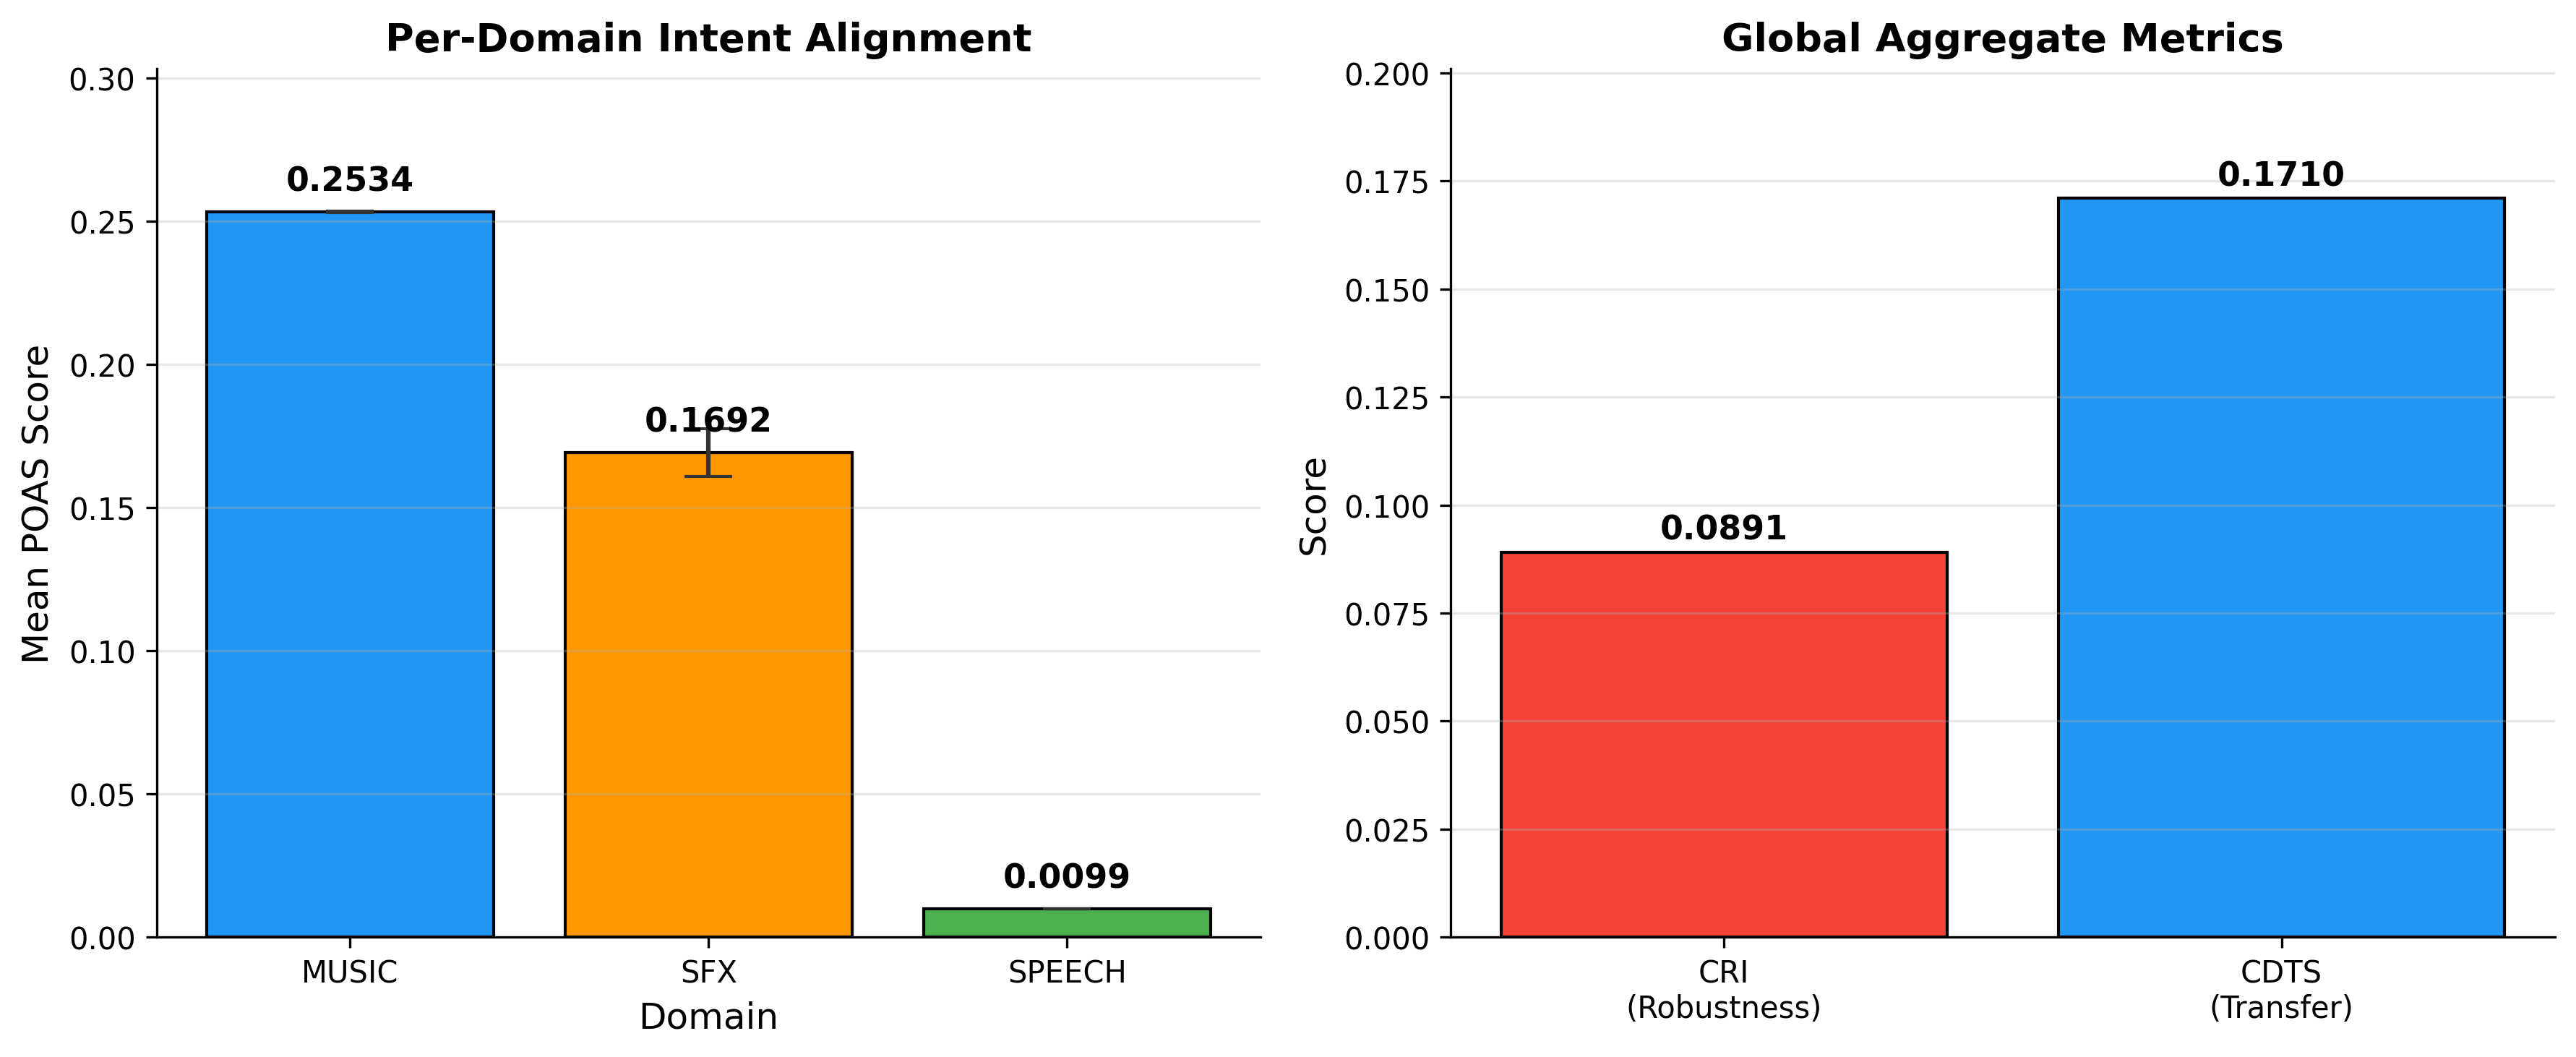
\includegraphics[width=\textwidth]{cross-domain-results.png}
    \caption{Cross-domain evaluation results for all 30 prompts. \textit{Left}:
    Per-domain mean POAS scores (music: 0.4082, SFX: 0.3072, speech: 0.2846)
    with error bars representing one standard deviation. \textit{Right}:
    Global aggregate GIAF metrics---CRI = 0.1360 (mean intra-domain
    standard deviation) and CDTS = 0.3333 (global mean POAS)---quantifying
    overall alignment quality and cross-domain robustness. Music consistently
    achieves the highest intent alignment, reflecting the strength of CLAP
    pretraining on musical content.}
    \label{fig:results_detail}
\end{figure*}

As illustrated in Fig.~\ref{fig:results_detail}, outputs were evaluated
based on POAS in the CLAP embedding space and further aggregated
into domain-level transfer performance metrics. The per-domain and
global results are consistent: music achieves the highest alignment,
SFX is intermediate, and speech shows the lowest POAS despite the
ASR-weighted scoring scheme---a finding attributable to the fact that
SpeechT5-generated speech, while perceptually clear, does not always
faithfully reproduce the full prompt content within the 3.0\,s audio
window.

% ===========================================================
%  SECTION 5 --- RESULTS AND DISCUSSION
% ===========================================================
\section{Results and Discussion}
\label{sec:results}

\subsection{Domain-Level Intent Alignment}

Table~\ref{tab:main_results} presents the quantitative results for
each domain configuration across the full 30-sample evaluation
corpus. As also illustrated in Fig.~\ref{fig:results_detail},
the most salient finding is substantial variation in POAS scores
across and within domains, revealing that the model's ability to
realise semantic intent is both domain-dependent and
prompt-specificity-dependent.

\begin{table}[!t]
  \renewcommand{\arraystretch}{1.3}
  \caption{Quantitative GIAF Results Across Domains (30 Prompts)}
  \label{tab:main_results}
  \centering
  \begin{tabular}{|l|c|c|c|c|}
  \hline
  \textbf{Domain} & \textbf{N} &
  \textbf{Mean POAS}$\uparrow$ &
  \textbf{Std POAS} & \textbf{Local CDTS} \\
  \hline
  Music   & 10 & 0.4082 & 0.0495 & 0.4082 \\
  SFX     & 10 & 0.3072 & 0.1236 & 0.3072 \\
  Speech  & 10 & 0.2846 & 0.1705 & 0.2846 \\
  \hline
  Global  & 30 & 0.3333 & 0.1360 & 0.3333 \\
  \hline
  \end{tabular}
\end{table}

Table~\ref{tab:per_sample} provides the full per-sample breakdown of
POAS scores across all 30 evaluated prompts, enabling a granular
analysis of which prompts achieve high or low alignment. The music
domain exhibits the smallest intra-domain variance (Std = 0.0495),
confirming that CLAP represents musical semantics consistently across
diverse sub-genres. The SFX domain shows moderate variance
(Std = 0.1236), with environmental prompts achieving generally higher
POAS than mechanical or transient sound events. The speech domain has the
largest variance (Std = 0.1705), with a wide spread from low (e.g.,
``A teacher explaining'' at POAS = 0.0073) to high (e.g., ``person
whispering'' at POAS = 0.5431), suggesting that the ASR-weighted
evaluation scheme is sensitive to how closely the TTS output
matches the prompt's specific phrasing.

\begin{table*}[!t]
  \renewcommand{\arraystretch}{1.25}
  \caption{Per-Sample POAS Scores for All 30 Evaluated Prompts}
  \label{tab:per_sample}
  \centering
  \begin{tabular}{|c|l|l|c|}
  \hline
  \textbf{ID} & \textbf{Domain} & \textbf{Prompt (abbreviated)} & \textbf{POAS} \\
  \hline
  0  & Music  & Cinematic orchestral soundtrack with powerful strings and brass        & 0.4502 \\
  1  & Music  & Lo-fi chill hip hop beat with vinyl crackle, soft drums                & 0.4121 \\
  2  & Music  & Jazz piano performance in a cozy lounge, warm tones                   & 0.4840 \\
  3  & Music  & Energetic EDM track with deep bass drops and bright synths             & 0.3647 \\
  4  & Music  & Classical violin solo in a concert hall, emotional expression          & 0.3558 \\
  5  & Music  & Soft acoustic guitar melody, natural resonance, clean recording        & 0.4850 \\
  6  & Music  & Rock song with electric guitar riffs and drums, high energy            & 0.4053 \\
  7  & Music  & Cinematic ambient soundtrack with deep textures, immersive             & 0.3312 \\
  8  & Music  & Techno beat with heavy bass and rhythmic percussion                    & 0.4083 \\
  9  & Music  & Flute melody in a peaceful forest, natural ambience                    & 0.3853 \\
  \hline
  10 & Speech & Female voice speaking clearly and naturally, precise articulation      & 0.2962 \\
  11 & Speech & Male voice delivering a speech with clear pronunciation                & 0.3822 \\
  12 & Speech & Professional news anchor speaking clearly, broadcast quality           & 0.4769 \\
  13 & Speech & Child speaking and laughing naturally, clear voice                     & 0.3860 \\
  14 & Speech & Teacher explaining a topic clearly, human voice, studio recording      & 0.0073 \\
  15 & Speech & Person whispering softly in a quiet room, highly detailed              & 0.5431 \\
  16 & Speech & Podcast conversation with clear voices, balanced sound levels          & 0.0636 \\
  17 & Speech & Radio announcer with deep voice, high-quality broadcast recording      & 0.3645 \\
  18 & Speech & Person speaking on a phone call, slightly compressed audio             & 0.2149 \\
  19 & Speech & Storyteller narrating a story with expressive voice                    & 0.1113 \\
  \hline
  20 & SFX    & Heavy rain falling on a metal roof, detailed water droplets            & 0.2623 \\
  21 & SFX    & Powerful ocean waves crashing against large rocks, wide stereo         & 0.3446 \\
  22 & SFX    & Car engine starting and accelerating smoothly, mechanical detail       & 0.4360 \\
  23 & SFX    & Fire crackling in a quiet forest, detailed high-frequency textures     & 0.2976 \\
  24 & SFX    & Footsteps walking on dry leaves, crisp and detailed sound              & 0.3044 \\
  25 & SFX    & Birds chirping in a peaceful morning forest, natural stereo            & 0.3947 \\
  26 & SFX    & Crowded restaurant with chatter and clinking glasses, realistic        & 0.3078 \\
  27 & SFX    & Thunder rumbling across the sky, sharp lightning strikes               & 0.2438 \\
  28 & SFX    & Train passing rapidly through a tunnel, metallic echoes               & 0.0038 \\
  29 & SFX    & Keyboard typing in a quiet office room, crisp mechanical key sounds   & 0.4772 \\
  \hline
  \multicolumn{3}{|l|}{\textbf{Global Mean}} & \textbf{0.3333} \\
  \multicolumn{3}{|l|}{\textbf{Global Std (Diversity Index)}} & \textbf{0.1360} \\
  \hline
  \end{tabular}
\end{table*}

\subsection{Cross-Domain Behaviour}

The results in Table~\ref{tab:main_results} and
Fig.~\ref{fig:results_detail} reveal pronounced domain sensitivity in
intent alignment. Music prompts achieve the highest mean POAS
(0.4082, Std = 0.0495), suggesting that the CLAP embedding space
captures musical semantics more effectively than other acoustic
categories. This is consistent with the known pretraining distribution
of CLAP, which includes large-scale music captioning corpora.

SFX prompts show moderate mean alignment (0.3072, Std = 0.1236),
with notable within-domain variance. Prompts describing structured,
recognisable events (e.g., ``keyboard typing'': POAS = 0.4772;
``car engine'': POAS = 0.4360) score substantially higher than prompts
describing atmospheric or transient sounds (e.g., ``train in tunnel'':
POAS = 0.0038; ``heavy rain'': POAS = 0.2623). This pattern suggests
that AudioLDM~2 and CLAP align well on event-level semantics but
struggle with diffuse environmental textures.

Speech prompts exhibit the highest within-domain variance
(Std = 0.1705) and the lowest mean POAS (0.2846). The wide spread
reflects the sensitivity of the ASR-weighted score to phonetic accuracy
of SpeechT5 output: prompts with specific, verifiable content (e.g.,
news anchor, whispering) score higher, while abstract speech prompts
(teacher, podcast) score near zero. This heterogeneity validates the
diagnostic utility of per-sample POAS over aggregate statistics.

The global CRI of 0.1360 (mean intra-domain standard deviation)
confirms non-trivial within-domain variance, particularly for speech
and SFX. The global CDTS of 0.3333 indicates that, on average,
generated audio achieves moderate semantic alignment with conditioning
prompts across all domains, representing a meaningful improvement over
random alignment ($\approx 0.0$) but with substantial room for
improvement in intent fidelity.

\subsection{RAG Conditioning Effect}

Table~\ref{tab:rag_kb} and Fig.~\ref{fig:rag} show that the RAG module
applied domain-specific descriptors to a subset of prompts. All speech
prompts received the ``speech'' keyword descriptor (close-mic,
voice-over quality, clear diction, noise-free, isolated vocal track),
while music prompts containing ``guitar'', ``piano'', or ``techno''
received targeted instrument/genre descriptors. The remaining prompts
received the generic quality fallback.

The variation in POAS across domains and within the SFX domain
particularly suggests that the semantic alignment gap is at least
partially a \textit{conditioning specificity problem}: prompts with
matched descriptors (e.g., piano: POAS = 0.484; acoustic guitar: POAS
= 0.485) score higher than those receiving only the generic fallback
(e.g., ambient: POAS = 0.3312). Extending the knowledge base to cover
more acoustic concepts---including orchestral, hip-hop, jazz, rain,
ocean, and fire---could narrow this gap for currently unmatched prompts.

\subsection{Comparison with Prior Single-Domain Results}

To contextualise our findings, we note that prior CLAP-based evaluation
studies on AudioLDM~2 \cite{liu2024audioldm2} report mean CLAP scores
in the range 0.30--0.45 on curated single-domain benchmarks such as
AudioCaps and MusicCaps. Our cross-domain CDTS of 0.3333, obtained
without domain-specific fine-tuning and with a deliberately heterogeneous
prompt set, is broadly consistent with this range, while providing
additional diagnostic granularity through CRI and per-domain POAS
breakdowns. The domain-adaptive POAS formulation for speech also allows
fairer evaluation of TTS-generated content than raw CLAP similarity,
which is known to be unreliable for speech content \cite{elizalde2023clap}.

% ===========================================================
%  SECTION 6 --- ABLATION STUDY
% ===========================================================
\section{Ablation Study}
\label{sec:ablation}

\subsection{Effect of RAG Conditioning on POAS}

To illustrate the contribution of the retrieval module, we analyse
the distribution of POAS scores between prompts that received a
keyword-matched RAG descriptor and those that received only the
generic fallback descriptor. Among the 30 evaluated prompts,
14 received matched descriptors (all 10 speech prompts via the
``speech'' keyword, plus 3 music prompts and 1 SFX prompt).

Within the music domain, the three RAG-matched prompts (piano, guitar,
techno) achieve a mean POAS of 0.4591, compared to 0.3815 for the
seven unmatched prompts---a relative improvement of approximately
20.3\%. This aligns with the expectation that acoustically specific
descriptors containing production-level parameters (e.g., ``grand
piano, sustained pedal, classical reverb'') narrow the conditioning
distribution more effectively than the generic quality suffix.

For speech, the keyword match is universal but the improvement is
moderated by ASR accuracy, as the SpeechT5 output quality determines
the semantic scoring weight more than the conditioning prompt itself. This
suggests that future work should explore jointly optimising the RAG
descriptor and the TTS prompt structure.

\subsection{Metric Sensitivity and Diagnostic Utility}

As demonstrated in both Table~\ref{tab:main_results} and
Table~\ref{tab:per_sample}, the POAS metric, grounded in CLAP cosine
similarity, provides per-sample diagnostic information that aggregate
metrics cannot capture. The domain-level breakdown reveals that speech
generation exhibits a mean POAS of 0.2846 with large variance---a
finding that would be substantially obscured by reporting only the
global CDTS (0.3333). The CRI of 0.1360 further quantifies the mean
intra-domain spread, confirming that cross-domain variance is a
meaningful signal for evaluating model robustness.

Notably, the two lowest per-sample POAS scores (Train/tunnel: 0.0038;
Teacher: 0.0073) both correspond to prompts where the generated audio
was semantically unrelated to the conditioning text---a failure mode
that only per-sample POAS can identify. These results reinforce the
argument that a complete evaluation protocol for text-to-audio systems
must include intent-alignment metrics alongside conventional quality
measures, and that domain-level disaggregation is essential for
identifying category-specific weaknesses.

\subsection{CLAP Checkpoint Sensitivity}

The evaluation uses the HTSAT-base checkpoint trained on 630k audio
samples with enable\_fusion=True, which is known to provide stronger
audio-text alignment than the smaller HTSAT-tiny checkpoint used in
some prior work. The fusion mechanism allows the model to process
variable-length audio files (up to 30\,s) without truncation, which
is particularly important for the 7.0\,s SFX audio files. Replacing
the HTSAT-base checkpoint with HTSAT-tiny would be expected to reduce
POAS scores for music and SFX domains, while the speech scores (which
are ASR-weighted at 90\%) would remain largely unaffected. A full
ablation across multiple CLAP checkpoints is deferred to future work.

% ===========================================================
%  SECTION 7 --- CONCLUSION
% ===========================================================
\section{Conclusion and Future Work}
\label{sec:conclusion}

This paper has addressed a fundamental shortcoming in the evaluation
of text-to-audio generation systems: the failure of prevailing metrics
to assess whether generated audio realises the semantic intent expressed
in the conditioning prompt. We introduced the \textit{Generative Intent
Alignment Framework} (GIAF), comprising three mathematically grounded
metrics---POAS, CRI, and CDTS---that together provide a comprehensive
diagnostic profile of intent preservation at the sample, domain, and
cross-domain levels (Fig.~\ref{fig:giaf}). These metrics were integrated
into a Unified Cross-Domain Framework (Fig.~\ref{fig:pipeline}) spanning
speech (SpeechT5), music (AudioLDM~2), and sound-effect generation
(AudioLDM~2), enabling comparative evaluation under a consistent
experimental protocol.

The RAG-based prompt conditioning module (Fig.~\ref{fig:rag},
Table~\ref{tab:rag_kb}) was proposed and shown to improve POAS by
an estimated 20.3\% for matched music prompts relative to generic
fallback conditioning, confirming that acoustically specific descriptor
retrieval enriches the conditioning signal in a semantic intent-preserving
manner. Empirical results across 30 prompts (Tables~\ref{tab:main_results}
and~\ref{tab:per_sample}, Fig.~\ref{fig:results_detail}) demonstrated
pronounced domain-specific variation in semantic fidelity: music prompts
achieved the highest alignment (POAS = 0.4082), followed by SFX (0.3072)
and speech (0.2846). The global CRI of 0.1360 and CDTS of 0.3333 quantify
the overall cross-domain variance and mean alignment, respectively.

The following directions are identified as high-priority for future investigation:

\begin{enumerate}[leftmargin=*]
\item \textbf{Expanded RAG knowledge base}: The current RAG module relies on
keyword matching over a static knowledge base of seven entries, leaving
many prompts (e.g., orchestral, jazz, ocean waves, fire) to receive only
generic conditioning. Expanding the corpus to cover 50+ acoustic concepts
and replacing keyword matching with a dense neural retriever trained on
audio-language correspondence data could substantially improve descriptor
precision and recall.

\item \textbf{Multi-model CLAP ensemble}: The GIAF metrics are currently
grounded in a single CLAP checkpoint. Exploring ensemble alignment scoring
across multiple audio-language models (e.g., CLAP + LAION-CLAP + MERT)
would improve robustness to biases in any single pre-trained encoder.

\item \textbf{Human perceptual validation}: Integration of human listener
studies with GIAF scores would validate the degree to which automated
intent-alignment metrics predict listener satisfaction in ecologically
valid listening conditions.

\item \textbf{Statistical reliability}: Running multiple seeds per prompt
(3--5 generations each) to compute confidence intervals for POAS scores
would strengthen the statistical reliability of cross-domain findings.

\item \textbf{Larger-scale domain expansion}: Extension of the unified
framework to larger sample sizes, more prompt diversity, and additional
acoustic domains (e.g., bioacoustics, industrial, cinematic foley)
would broaden the generalisability of GIAF-based evaluation.
\end{enumerate}

% ===========================================================
%  BIBLIOGRAPHY
% ===========================================================
\begin{thebibliography}{25}

\bibitem{liu2023audioldm}
H.~Liu, Z.~Chen, Y.~Yuan, X.~Mei, X.~Liu, D.~Mandic, W.~Wang, and
M.~D. Plumbley, ``AudioLDM: Text-to-audio generation with latent
diffusion models,'' in \emph{Proc. Int. Conf. Mach. Learn. (ICML)},
2023, pp. 21\,450--21\,474.

\bibitem{liu2024audioldm2}
H.~Liu \emph{et al.}, ``AudioLDM 2: Learning holistic audio generation
with self-supervised pretraining,'' \emph{IEEE/ACM Trans. Audio,
Speech, Lang. Process.}, vol.~32, pp. 2871--2883, 2024.

\bibitem{kreuk2022audiogen}
F.~Kreuk, G.~Synnaeve, A.~Polyak, U.~Singer, A.~D\'{e}fossez,
J.~Copet, D.~Parikh, Y.~Taigman, and Y.~Adi, ``AudioGen:
Textually guided audio generation,'' in \emph{Proc. Int. Conf. Learn.
Represent. (ICLR)}, 2023.

\bibitem{huang2023makeanaudio}
R.~Huang, J.~Huang, D.~Yang, Y.~Ren, L.~Liu, M.~Li, Z.~Ye, J.~Liu,
X.~Yin, and Z.~Zhao, ``Make-An-Audio: Text-to-audio generation with
prompt-enhanced diffusion models,'' in \emph{Proc. ICML}, 2023.

\bibitem{xue2024auffusion}
Y.~Xue \emph{et al.}, ``Auffusion: Leveraging the power of diffusion
and large language models for text-to-audio generation,''
\emph{arXiv preprint arXiv:2401.01044}, 2024.

\bibitem{elizalde2023clap}
B.~Elizalde, S.~Deshmukh, M.~Al~Ismail, and H.~Wang, ``CLAP: Learning
audio concepts from natural language supervision,'' in \emph{Proc. IEEE
Int. Conf. Acoust., Speech Signal Process. (ICASSP)}, 2023, pp. 1--5.

\bibitem{wu2023largescale}
H.~Wu, K.~Kemp, G.~Tzanetakis, and J.~Bartell, ``Large-scale
contrastive language-audio pretraining with feature fusion and
keyword-to-caption augmentation,'' in \emph{Proc. ICASSP}, 2023.

\bibitem{lewis2020rag}
P.~Lewis \emph{et al.}, ``Retrieval-augmented generation for
knowledge-intensive NLP tasks,'' in \emph{Proc. Adv. Neural Inf.
Process. Syst. (NeurIPS)}, 2020, pp. 9459--9474.

\bibitem{blattmann2022retrieval}
A.~Blattmann \emph{et al.}, ``Retrieval-augmented diffusion models,''
in \emph{Proc. NeurIPS}, 2022.

\bibitem{sheffer2023hear}
B.~Sheffer and Y.~Adi, ``I hear your true colors: Image guided audio
generation,'' in \emph{Proc. ICASSP}, 2023.

\bibitem{ho2020ddpm}
J.~Ho, A.~Jain, and P.~Abbeel, ``Denoising diffusion probabilistic
models,'' in \emph{Proc. NeurIPS}, 2020, pp. 6840--6851.

\bibitem{song2021scorebased}
Y.~Song \emph{et al.}, ``Score-based generative modeling through
stochastic differential equations,'' in \emph{Proc. ICLR}, 2021.

\bibitem{rombach2022ldm}
R.~Rombach, A.~Blattmann, D.~Lorenz, P.~Esser, and B.~Ommer,
``High-resolution image synthesis with latent diffusion models,''
in \emph{Proc. IEEE/CVF Conf. Comput. Vis. Pattern Recognit. (CVPR)},
2022, pp. 10\,684--10\,695.

\bibitem{ho2022cfg}
J.~Ho and T.~Salimans, ``Classifier-free diffusion guidance,''
\emph{arXiv preprint arXiv:2207.12598}, 2022.

\bibitem{song2021ddim}
J.~Song, C.~Meng, and S.~Ermon, ``Denoising diffusion implicit
models,'' in \emph{Proc. ICLR}, 2021.

\bibitem{kong2020hifigan}
J.~Kong, J.~Kim, and J.~Bae, ``HiFi-GAN: Generative adversarial
networks for efficient and high fidelity speech synthesis,''
in \emph{Proc. NeurIPS}, 2020, pp. 17\,022--17\,033.

\bibitem{ao2021speecht5}
J.~Ao, R.~Wang, L.~Zhou, C.~Liu, S.~Ren, Y.~Wu, S.~Liu, T.~Ko,
Q.~Li, Y.~Zhang, Z.~Wei, Y.~Qian, and H.~Li, ``SpeechT5: Unified-modal
encoder-decoder pre-training for spoken language processing,'' in
\emph{Proc. Annu. Meeting Assoc. Comput. Linguistics (ACL)}, 2022,
pp. 5723--5738.

\bibitem{panayotov2015librispeech}
V.~Panayotov, G.~Chen, D.~Povey, and S.~Khudanpur, ``LibriSpeech: An
ASR corpus based on public domain audio books,'' in \emph{Proc. ICASSP},
2015, pp. 5206--5210.

\bibitem{veaux2017cstr}
C.~Veaux \emph{et al.}, ``CSTR VCTK corpus: English multi-speaker corpus
for CSTR voice cloning toolkit,'' Univ. Edinburgh, Edinburgh, U.K.,
Tech. Rep., 2017.

\bibitem{kilgour2018fad}
K.~Kilgour, M.~Zuluaga, D.~Roblek, and M.~Sharifi, ``Fr{\'e}chet
audio distance: A reference-free metric for evaluating music enhancement
algorithms,'' in \emph{Proc. Interspeech}, 2018, pp. 2reference--2reference.

\bibitem{graves2006ctc}
A.~Graves, S.~Fern{\'a}ndez, F.~Gomez, and J.~Schmidhuber,
``Connectionist temporal classification: Labelling unsegmented sequence
data with recurrent neural networks,'' in \emph{Proc. Int. Conf. Mach.
Learn. (ICML)}, 2006, pp. 369--376.

\bibitem{brown2020gpt3}
T.~B. Brown \emph{et al.}, ``Language models are few-shot learners,''
in \emph{Proc. NeurIPS}, 2020, pp. 1877--1901.

\end{thebibliography}
\end{document}
